\let\negmedspace\undefined
\let\negthickspace\undefined
\documentclass[journal]{IEEEtran}
\usepackage[a5paper, margin=10mm, onecolumn]{geometry}
%\usepackage{lmodern} % Ensure lmodern is loaded for pdflatex
\usepackage{tfrupee} % Include tfrupee package

\setlength{\headheight}{1cm} % Set the height of the header box
\setlength{\headsep}{0mm}     % Set the distance between the header box and the top of the text

\usepackage{gvv-book}
\usepackage{gvv}
\usepackage{cite}
\usepackage{amsmath,amssymb,amsfonts,amsthm,mathtools}
\usepackage{algorithmic}
\usepackage{graphicx}
\usepackage{textcomp}
\usepackage{xcolor}
\usepackage{txfonts}
\usepackage{listings}
\usepackage{enumitem}
\usepackage{mathtools}
\usepackage{gensymb}
\usepackage{comment}
\usepackage[breaklinks=true]{hyperref}
\usepackage{tkz-euclide} 
\usepackage{listings}
\def\inputGnumericTable{}                                 
\usepackage[latin1]{inputenc}                                
\usepackage{color}                                            
\usepackage{array}                                            
\usepackage{longtable}                                       
\usepackage{calc}                                             
\usepackage{multirow}                                         
\usepackage{hhline}                                           
\usepackage{ifthen}                                           
\usepackage{lscape}
\begin{document}

\bibliographystyle{IEEEtran}
\vspace{3cm}

\title{1.11.7}
\author{EE24BTECH11001 - Aditya Tripathy
}
% \maketitle
% \newpage
% \bigskip
{\let\newpage\relax\maketitle}

\renewcommand{\thefigure}{\theenumi}
\renewcommand{\thetable}{\theenumi}
\setlength{\intextsep}{10pt} % Space between text and floats

\textbf{Question:}\\
Construct an equilateral triangle ABC with each side 5cm.
\\
\textbf{Solution:}\\
Let $\vec{A}$ = $\vec{0}$, and $\vec{B}$ = \myvec{5\\0}. $\vec{C}$ is the required vertex.\\ Since the triangle is equilateral,
\begin{align}
    \vec{C} = R\brak{\vec{B-A}}\\
    R = \myvec{\cos \frac{\pi}{3} & -\sin \frac{\pi}{3} \\ \sin \frac{\pi}{3} & \cos \frac{\pi}{3}}
\end{align}
where R is the rotation matrix which rotates the vector $\vec{B-A}$ by angle $\frac{\pi}{3}$. On calculation,
\begin{align}
    \vec{C} = \myvec{\frac{1}{2} & -\frac{\sqrt{3}}{2}\\ \frac{\sqrt{3}}{2} & \frac{1}{2}} \myvec{5\\0}\\
    \vec{C} = \myvec{\frac{5}{2} \\ \frac{5\sqrt{3}}{2}}
\end{align}
\begin{figure}[h!]
   \centering
   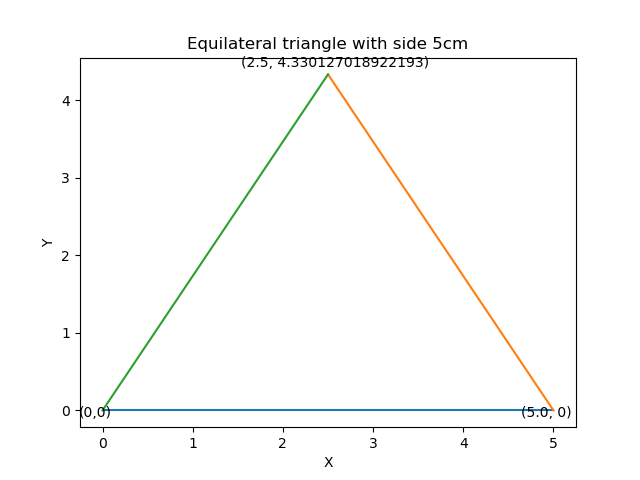
\includegraphics[width=0.7\linewidth]{figs/fig.png}
   \caption{equilateral triangle of side 5cm}
\end{figure}

\end{document}
